\documentclass{article}
\usepackage{pdfpages}

\begin{document}
\thispagestyle{empty} 

\noindent
This is an introduction to IPython which I recently wrote. It is intended for
Advanced Lab students, and addresses the problem that while practicing
physicists need basic programming skills, our students have a huge range of
computational backgrounds. We now have students solve the practical problems of
data management and analysis in IPython, so that everyone gains some exposure to
the subject. My hope is that this document is an essential introduction for
novices, a reference for those learning, and unobstructive to the
skilled. Future versions will have better integration with the material on
confidence testing and data analysis techniques.

\vfill 
\newpage
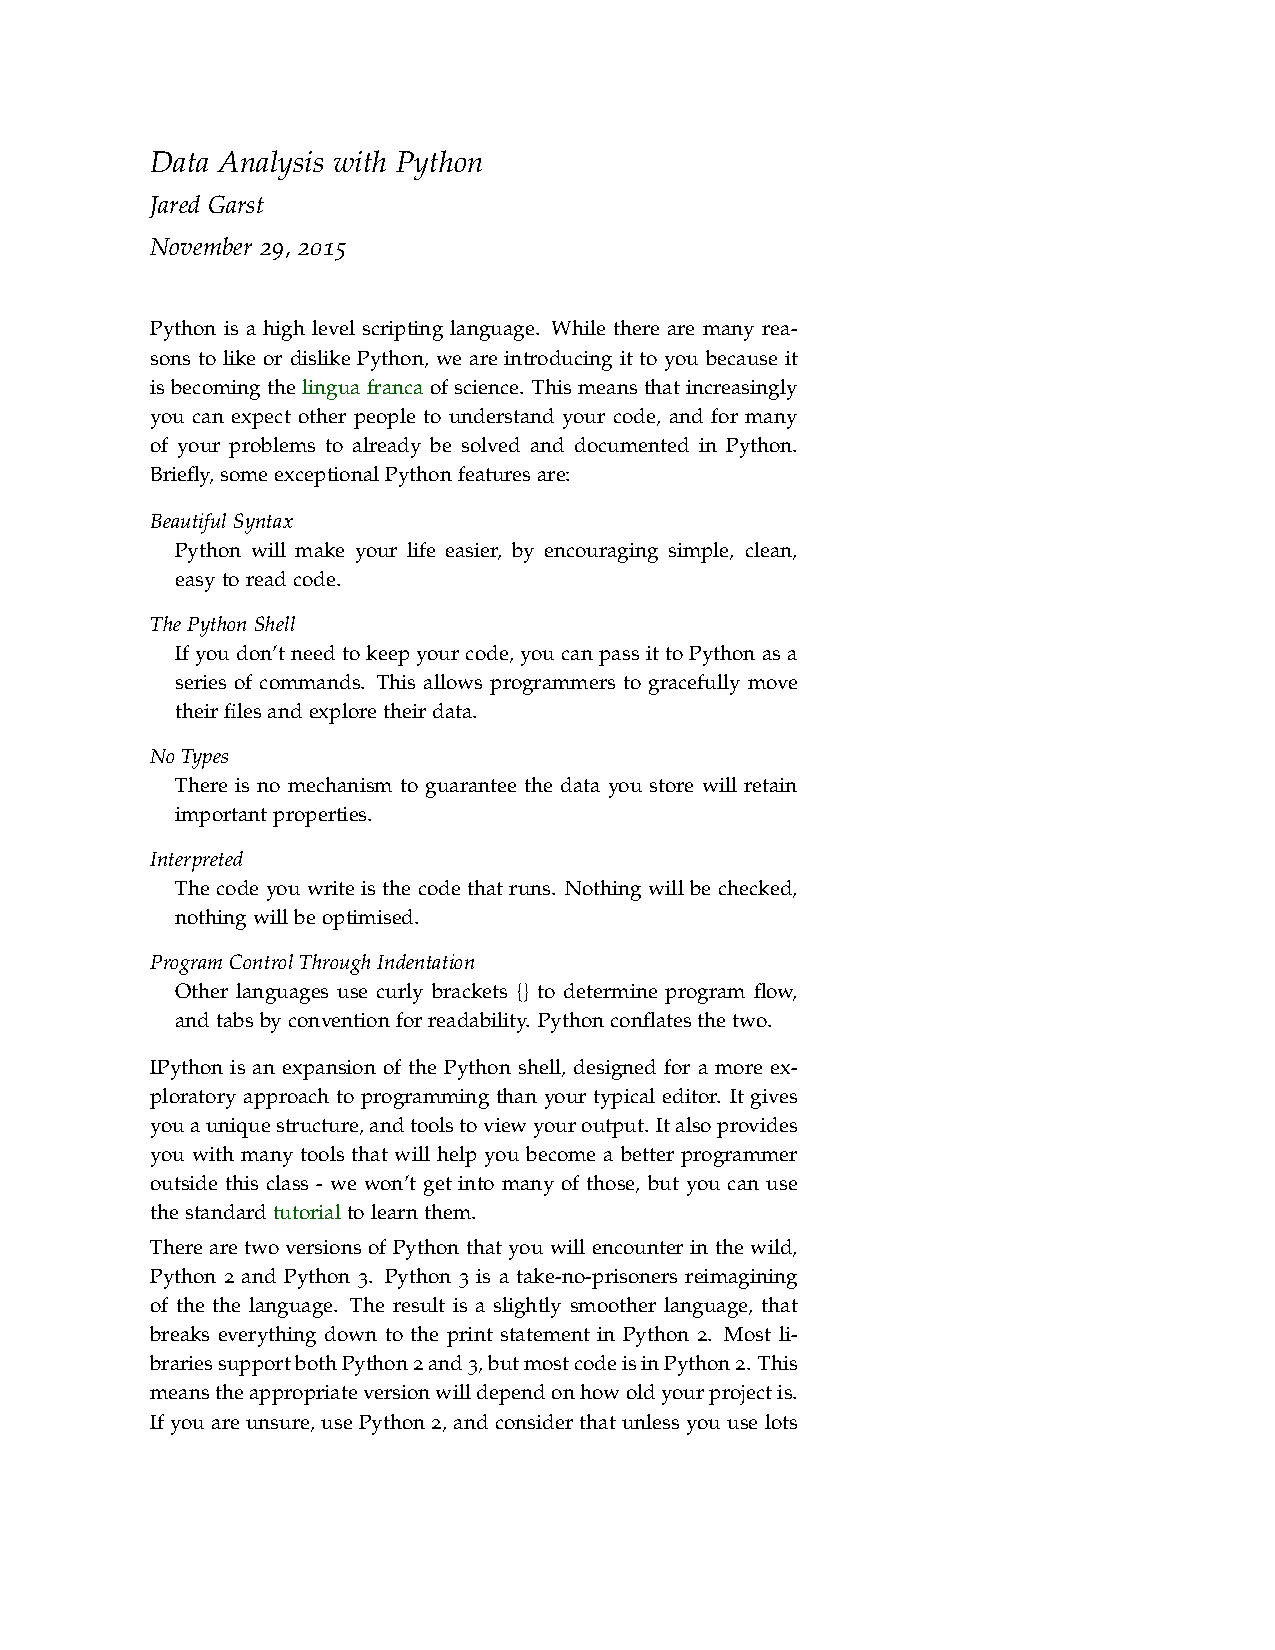
\includepdf[pages=1-, pagecommand={\thispagestyle{empty}}]{ClassMaterials/Python-FirstSteps}

\end{document}